\documentclass{beamer}

\usetheme{CambridgeUS}
\usecolortheme{beaver}

\setlength{\parskip}{\baselineskip}

\title{Fault Tolerance in Block-Level Caching}
\author{
  Jesus Ramos \and
  Douglas Otstott
}
\institute[FIU]{Florida International University}
\date{}

\begin{document}

\maketitle

\section{Problem Description}

\subsection{Problem Statement}

\begin{frame}
  \frametitle{Problem Statement}

Fault tolerance in warehouse scale systems is an important issue
-Expect faults to happen
-Deal with faults online

Systems need to be: 
-dependable and reliable
-able to handle failure quickly and effectively

\end{frame}

% end subsection Problem Statement

\subsection{Background}

\begin{frame}
  \frametitle{Problem Background}
%To do - add bullets
Warehouse Scale Computing Architecture utilizes Storage Area Networks for persistant storage
-Increase reliablity
-Easy to Mirgrate VMs
-Storage Bandwidth = Performance Bottleneck %can we make this red to indicate it is a drawback?

Storage Area Networks use Cache
-Leverages Network Storage
-Large Performance Increase
-Reduced fault tolernace %also make this red if possible

\end{frame}

\begin{frame}
  \frametitle{Problem Background}
  \begin{center}
    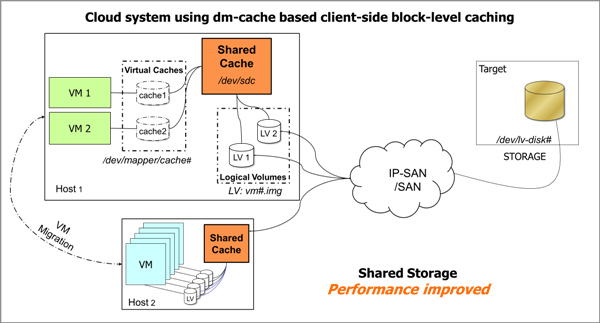
\includegraphics[scale=0.85]{../Images/NewerImage.png}
  \end{center}

Cache device on host machine
-Virtual mapping between virtual disk and central storage

\end{frame}

\begin{frame}
  \frametitle{DM-Cache}

DM-Cache
-open source block level (Linux Kernel module) caching solution
-allows host machines to store recently used blocks
-reduces the number of requests to central storage systems.

Increases performance
-access time must less than cental storage
-greatly reduces contension for network storage

Decreases Fault Tolerance
-Metadata is non persistnt
-Writes are buffered through the cache
-local modifications temporarily vulnerable

\end{frame}

% end subsection Background

% end section Problem Description

\section{Proposed Solution}

\subsection{Metadata Persistence}

\begin{frame}
  \frametitle{Persist the Metadata}

Solution:
-move the non-persistent metadata from to the persistent cache device
   -Facilitates the reconstruction of the cache
-metadata to be cached in memory
   -written back to disk via background process
	-trade offs of write back methods

\end{frame}

% end subsection Metadata Persistence

% end section Proposed Solution

\section{Project Timeline}

\begin{frame}
  \frametitle{Tentative Timeline}
  \begin{description}
    \item[February 26th] - Begin Preliminary Testing (Radix Tree)
    \item[March 1st] - Begin solution implementation (Radix/Hash)
    \item[April 5th] - Debug solution (Hash Table)
    \item[April 10th] - Begin Evaluation
    \item[April 15th] - Conclude Evaluation
    \item[April 20th] - Write a paper and presentation
  \end{description}
\end{frame}

% end section Project Timeline

\section{Project Evaluation}

\begin{frame}
  \frametitle{Evaluation Criteria}

  In this project we will evaluate the following:
  \begin{itemize}
    \item The run-time overhead of two persistence techniques for
    metadata
	-updating the metadata in the background while keeping it cached on the disk
	-forcing a write back every time the metadata changes
    \item The amount of time it takes to restore a cache to its last
    persistence point before the system failure

    \item The amount of data that can be recovered using both techniques

    \item The trade-offs between both techniques 
		-data can be recovered
		-run time overhead
  \end{itemize}

\end{frame}

% end section Project Timeline

\section{Questions}

\begin{frame}
  \frametitle{Questions?}
\end{frame}

% end section Questions

\end{document}
